\documentclass{article} % For LaTeX2e
\usepackage{nips15submit_e,times}
\usepackage{hyperref}
\usepackage{url}
\usepackage{lipsum}
\usepackage{graphicx}
\usepackage{amssymb}
\usepackage{amsmath}
\usepackage{amsthm}
\usepackage{alltt}
\usepackage{float}
\usepackage{color}
\usepackage{listings}
\usepackage{multicol}

\usepackage[a4paper, portrait, margin=1in]{geometry}

\newcommand{\tab}{\hspace*{2em}}

\lstset{ %
   language=Python,                % choose the language of the code
   basicstyle=\small,        % the size of the fonts that are used for the code
   keywordstyle=\color{blue},
   stringstyle=\color{red},
   commentstyle=\color{green},
   numbers=left,                   % where to put the line-numbers
   numberstyle=\footnotesize,      % the size of the fonts that are used for the line-numbers
   stepnumber=1,                   % the step between two line-numbers. If it is 1 each line will be numbered
   numbersep=5pt,                  % how far the line-numbers are from the code
   backgroundcolor=\color{white},  % choose the background color. You must add \usepackage{color}
   showspaces=false,               % show spaces adding particular underscores
   showstringspaces=false,         % underline spaces within strings
   showtabs=false,                 % show tabs within strings adding particular underscores
   frame=single,           % adds a frame around the code
   tabsize=2,          % sets default tabsize to 2 spaces
   captionpos=b,           % sets the caption-position to bottom
   breaklines=true,        % sets automatic line breaking
   breakatwhitespace=false,    % sets if automatic breaks should only happen at whitespace
   escapeinside={\%*}{*)}          % if you want to add a comment within your code
   }



% The \author macro works with any number of authors. There are two commands
% used to separate the names and addresses of multiple authors: \And and \AND.
%
% Using \And between authors leaves it to \LaTeX{} to determine where to break
% the lines. Using \AND forces a linebreak at that point. So, if \LaTeX{}
% puts 3 of 4 authors names on the first line, and the last on the second
% line, try using \AND instead of \And before the third author name.
\author{
Evan Steele \\
Student \\
Address \\
\texttt{steelee@gmail.com} \\
}
\newcommand{\fix}{\marginpar{FIX}}
\newcommand{\new}{\marginpar{NEW}}

\title{Applying Machine Learning to League of Legends Ranking Data}
\author{Evan Steele \and Darren Marshall \and Jacob Mastel}
\begin{document}
\begin{titlepage}
   \vspace*{\stretch{1.0}}
   \begin{center}
      \Large\textbf{Applying Machine Learning to League of Legends Ranking Data}\\
      \large\textit{Evan Steele, Darren Marshall, and Jacob Mastel}
   \end{center}
   \vspace*{\stretch{2.0}}
\end{titlepage}
\section{Abstract}
League of Legends incorporates complex metrics to determine how players rank in the Leagues system for online competitive matchmaking. We experimented with a large dataset of player metrics and rank information to determine how accurately we could assess player rank given a feature set of their ranked season performance. We used an implementation of ranking via pairwise transform and SVMs from the MLPY library and a more standard linear regression implementation. We will show this information visually and through code to demonstrate our result and assess how accurately we can make these predictions.


\section{Introduction}
\subsection{Background}
\subsubsection{League of Legends}
League of Legends (also abbreviated as LoL) is an online multiplayer video game, with about 67 million active players across the world, making it the most played game in the world \cite{statista}. Players form two teams of five, and then pick from a list of 131 unique characters, each with a unique set of abilities. Each match is discrete, with all players starting off fairly weak, but growing in strength throughout a game through the acquisition of experience and gold to purchase items. The teams then try to attack the opposing team and invade their base to destroy a central structure, which is guarded by various defenses and the enemy team.\\

The average game lasts between 35 and 45 minutes, so matching players up based on skill is crucial for a balanced game. The game uses an intricate ranking system to place players in specific tiers of competition. The matchmaking system then places similar players into teams 

\subsubsection{Ranking System}
Among the most influential factors in LoL's success is its tiered ranking system in which players are placed into seven tiers of skill \cite{lolpopular}. This way each game is roughly evenly matched and players can play a "fair" game. A player in Bronze tier should be matched against mostly Bronze players, and maybe a few Silver players. Then if they win the game their rank is increased (decreased if they lose) until one day they are promoted to the Silver tier, and up the ladder through Gold, Platinum, Diamond, Master, and Challenger. These ranks should provide a summary of performance for the matchmaking system. Typically, the system requires 10 games of "calibration" to be completed before a ranking is assigned. Using other games across other players of various tiers, what can we learn about successfully ranking a new set of players?

\begin{figure}[h!]
\centering
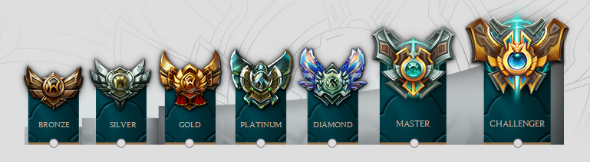
\includegraphics[scale=0.7]{tiers.png}
\caption{The seven tiers in League of Legends}
\label{fig:univerise}
\end{figure}

\subsection{Our challenge: Predict a player's tier based on their performance}
Where does a player belong? We can see what tier they are in right now, but what tier should they be in based on their objective performance? Is a bronze player playing like a Gold player? Is there a Gold player that's out of touch and is playing like a Silver player? If you were able to look at all the games a player has played, will we find that they are similar to the other players in their tier, or will we find they are playing more like players in other tiers?


\subsection{Significance}

\subsubsection{A player's rank is a form of social status}
Because a tier represents a player's ability to play the game there is huge social status attached to each tier; so much so that as a general rule all players, especially Bronze players, assume they belong in at least the next highest tier, if not two tiers up. Perhaps this is true, but perhaps by looking at factual data we can determine that this is a purely psychological phenomena and not accurate.

\subsubsection{Ranking systems in modern games}
LoL is the most popular video game today, making it arguably the most successful. Naturally other game companies will mimic the ranking system in LoL in hopes of finding the same level of success. Indeed there are several examples of AAA games that have adopted a very similar ranking system. Examples include Starcraft 2, Call of Duty, and Clash of Clans. Efforts made to understand and apply LoL's ranking system will lead to a better understanding of this aspect of all competitive modern multiplayer games.


\section{Proposed approach}
We formulated the problem as a supervised learning task. We could get all our testing and training data including labels through the LoL API. We decided to use two machine learning algorithms to conduct our experiment: ranking and linear regression.

\subsubsection{Why choose a ranking algorithm?}
We chose ranking because the problem lends itself to the idea of selecting an order of things. Which tier does this player fit in? That can be answered by lining everybody up in order of best to worst and then choosing thresholds.

\subsubsection{Why choose a linear regression algorithm?}
We chose linear regression as our second algorithm to learn placement because we expect player's performance to evolve over time. Higher values of one variable or another might be indicative of higher or lower tier performance.

\subsection{Data harvesting}
Since LoL supports a developer API, we were able to access hoards of data from real games. This data included a breakdown of each player's total lifetime statistics, including what rank they are in, how many games they have played total, how many times they played each champion, exactly how much damage each champion has dealt total, and a host of other useful information. We chose to use the "seed data" available publicly by Riot. This data consists of 1000 randomly-selected recent matches from the North American server. We chose 2400 players randomly from the 1000 matches. Then we used Riot's API to get both the rank and complete statistics of these 2400 players.

\subsubsection{Retrieval}
We retrieved the data using the Riot Games API, requiring two API calls per user. Our generation process for this data set had to be original, since a raw set of player data for our purposes did not exist yet. To get the format we wanted, we needed to perform these steps:
\begin{itemize}
  \item Usage for \textit{gendata.py}
  \begin{itemize}
    \item Get seed file containing 1000 random ranked matches
    \item extract 5 random player IDs (out of 10) per match
  \end{itemize}
  \item Request player data for matches
  \item Add up ranked stats, average them using total number of champions played
  \item Request player data for given rank
  \item Write data to features and target files
\end{itemize}


\subsection{Feature selection}
We selected thirteen specific features from the myriad of information based on what we assumed would be relevant to standard play on a normal Summoner's Rift game. For example, we removed all statistics that only dealt with Dominion games. Then we chose the thirteen most relevant variables: totalPhysicalDamageDealt, totalTurretsKilled, totalSessionsPlayed, totalAssists, totalDamageDealt, totalDeathsPerSession, totalSessionsWon, totalGoldEarned, totalChampionKills, totalMinionKills, totalSessionsLost, totalDamageTaken, and totalMagicDamageDealt.

We left out variables we determined to be least helpful in predicting rank, such as the number of Bot games played, the largest killing spree on a particular champion, and the largest critical strike.


\subsection{A look at the data}
Upon inspection of the data, we have a surprisingly diverse selection of players, the largest represented category being Silver, at 39%.

\begin{figure}[h!]
\centering
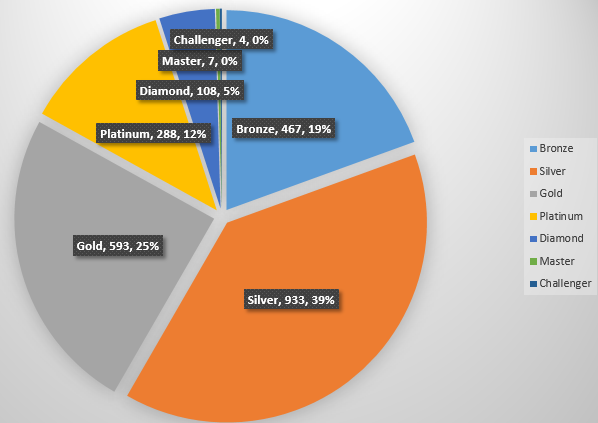
\includegraphics[scale=0.9]{tiers-pie.png}
\caption{A breakdown of our data by tier}
\label{fig:univerise}
\end{figure}

A quick graph of the data in various ways pulled a bit of understanding before we approached the programming. There appears to be a linear correlation between the win percentage and the tier.

\begin{figure}[h!]
\centering
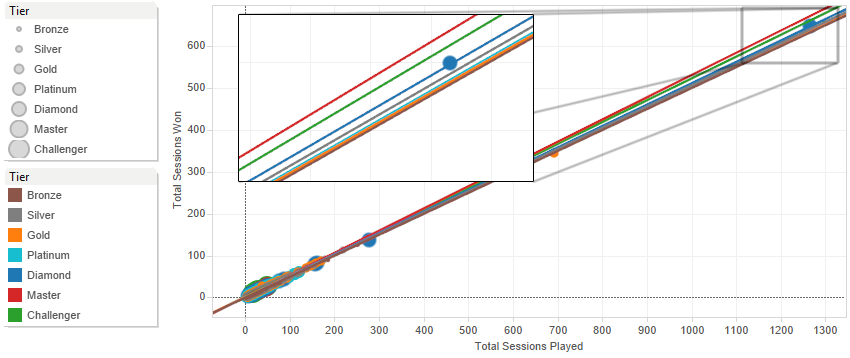
\includegraphics[scale=0.7]{win_percentage.png}
\caption{A linear correlation between win percentage and tier, with the highest tiers standing out by far.}
\label{fig:univerise}
\end{figure}

\subsection{Pre-processing}
The raw data from the API came with extra variables that were not included in our feature set. It was also grouped into player and champion statistics. In order to aggregate the data into a single list of 13 features per player that represented the player's performance, we calculated the average values per champion.




\section{Experiments}

\subsection{Ranking Algorithm}

\subsubsection{Software package: Scikit-learn}
Scikit-learn is a machine learning package in Python which provides simple and efficient tools for data mining and data analysis.

We used Scikit-learn's Itertools algorithm to implement leave-one-out cross validation on our training set.




\subsection{Linear Regression Algorithm}


The software package we chose for our Linear Regression algorithm was Numpy and Statsmodels. We were already familiar with Numpy, and Statsmodels was recommended by an expert.



\subsection{Linear Regression Algorithm}
The linear regression algorithm uses the python package, statsmodel. Statmodel's object, OLS, was used in conjunction with a 2,000 sample training set. That gave us a weight vector that could then be compared against a testing set of 400 samples. The code listed below is an abbreviated version of the application used.
\begin{lstlisting}
x,y = build_matricies('train')
model   = sm.OLS(y, x)
results = model.fit_regularized()
weights = results.params
pred    = model.predict(weights)
summary = results.summary().as_text()
f.write(summary)
x,y = build_matricies('test')
for i in range(x.shape[0]):
	val = int(numpy.round(numpy.dot(weights, x[i])))
	yv  = int(y[i])
	if val == yv:
		success += 1
	else:
		failure += 1
total           = success + failure
percent_correct = int((float(success) / float(total)) * 100)
print "{0}\t{1}\t{2}\t{3}%".format(success, failure, total, percent_correct)
placement_matrix = numpy.zeros((7,7), dtype=numpy.int)
for i in range(x.shape[0]):
	val = int(numpy.round(numpy.dot(weights, x[i])))
	placement_matrix[int(y[i]),val] += 1
print placement_matrix
\end{lstlisting}


\subsection{Ranking Algorithm}
The ranking algorithm uses the RankSVM class from the MLPY library \cite{mlpy} to actually create the data. After formatting the data, we applied the pairwise tranformation method, to bring each data set of 13 features to a 2D graph point. The result of processing this used this function:\\
\begin{lstlisting}
def transform_pairwise(X, y):
    X_new = []
    y_new = []
    y = np.asarray(y)
    if y.ndim == 1:
        y = np.c_[y, np.ones(y.shape[0])]
    comb = itertools.combinations(range(X.shape[0]), 2)
    for k, (i, j) in enumerate(comb):
        if y[i, 0] == y[j, 0] or y[i, 1] != y[j, 1]:
            continue
        X_new.append(X[i] - X[j])
        y_new.append(np.sign(y[i, 0] - y[j, 0]))
        if y_new[-1] != (-1) ** k:
            y_new[-1] = - y_new[-1]
            X_new[-1] = - X_new[-1]
    return np.asarray(X_new), np.asarray(y_new).ravel()
\end{lstlisting}
This library will attempt to rank players by rank, assigning players to groups based on how they rank against each other. We placed them into groups based on the valid ranks we assigned in the target file, which was an interger between 0 and 6. The result looks like this:\\

\begin{figure}[h!]
\centering
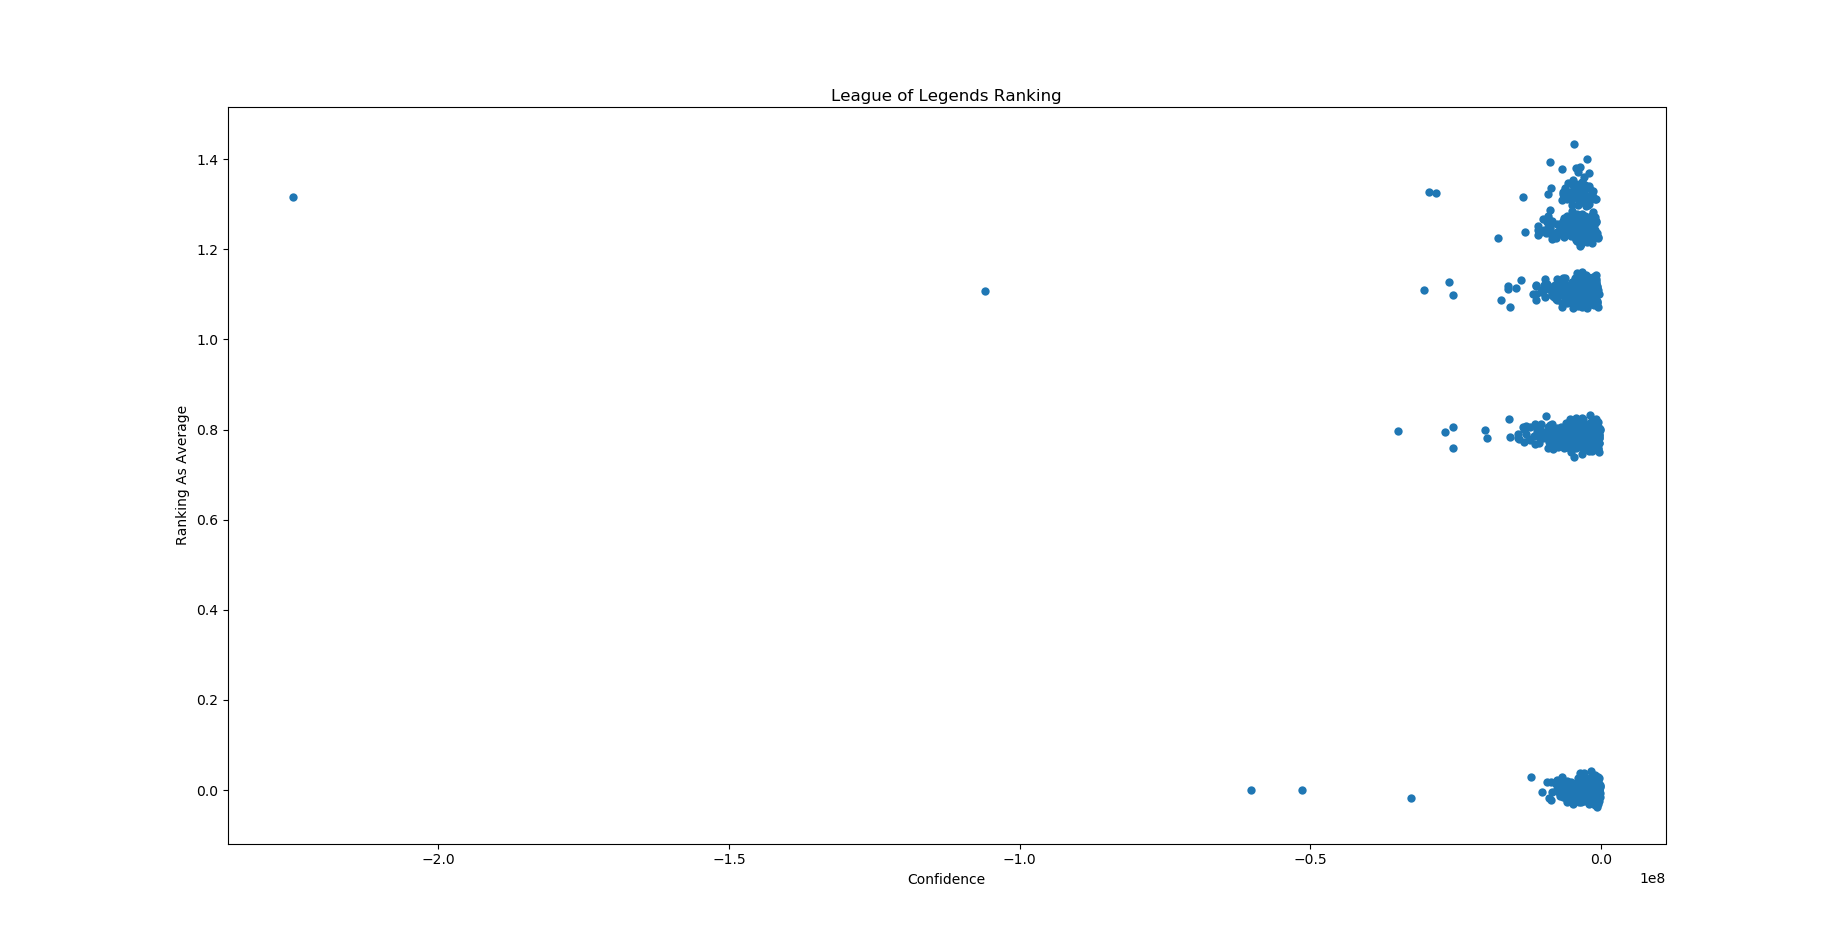
\includegraphics[scale=0.35]{ranking_regression.PNG}
\caption{Ranking regression result}
\label{fig:ranking}
\end{figure}

\subsubsection{Chosen software package for our RidgeCV linear regression Algorithm: Scikit-learn}
We found a third algorithm that was easy to implement as a third option. Scikit-learn came packaged with a linear regression algorithm called RidgeCV. This implemented ridge regression with leave-one-out cross-validation, and was useful for us to implement because of multi-colinearality of the data.

\section{Results}
We had no real baselines to work with with regards to this data, since we were using a set of player data averaged over number of unique champions played, rather than just the total number of games played. We hypothesised that it would provide us better data with regards to ranking. The design for these two algorithms came right from their respective tool-sets.

\subsection{Ranking Algorithm}
The ranking algorithm showed results that were not as conclusive as we were expecting. Our results were showing a limited success rate in classification, as noted by the accuracy report:
\begin{lstlisting}
Performance of ranking  0.444810126582
Performance of linear regression  0.564185463659
Real placement ratios in file:
{0: 0.1765, 1: 0.391, 2: 0.2635, 3: 0.126, 4: 0.039, 5: 0.003, 6: 0.001}
\end{lstlisting}

\subsection{Linear Regression Algorithm}
Our experiments with linear regression showed little, if any, significant results. The regression analysis produced an $R^2$ value of 0.262. Checking its correctness against a testing set demonstrated that the derived function is only 39\% accurate.

\begin{table}[]
\centering
\caption{Linear Regression tier predictions versus actual predictions}
\label{my-label}
\begin{tabular}{llllllll}
\multicolumn{1}{c}{} & \multicolumn{7}{c}{Our Predictions}                               \\
\textbf{Actuals}     & Bronze & Silver & Gold & Platinum & Diamond & Master & Challenger \\
\textbf{Bronze}      & 14     & 91     & 7    & 0        & 1       & 1      & 1          \\
\textbf{Silver}      & 0      & 100    & 49   & 1        & 0       & 1      & 0          \\
\textbf{Gold}        & 0      & 24     & 40   & 1        & 1       & 0      & 0          \\
\textbf{Platinum}    & 0      & 5      & 30   & 1        & 0       & 0      & 0          \\
\textbf{Diamond}     & 0      & 4      & 18   & 7        & 1       & 0      & 0          \\
\textbf{Master}      & 0      & 0      & 1    & 0        & 0       & 0      & 0          \\
\textbf{Challenger}  & 0      & 0      & 1    & 1        & 0       & 0      & 0         
\end{tabular}
\end{table}

\subsection{Conclusions}
% What conclusions do you draw from the results? 

We have concluded that a linear regression creates an inherently bad fit for our problem. We believe this is primarily caused by the fact that the different tiers have an uneven weight by design. This uneven weight seems to strongly bias the function away from predicting members of the bronze tier, for example. Instead, it shifts data points of all tiers towards silver and gold.

\section{Insights}
The low accuracy rate indicates that linear regression may not have been the best choice in this circumstance. League of Legends is an extremely complicated game, with a huge number of variables that all converge in wild ways. We need an algorithm that is able to show the combination of variables in specific instances, rather than a conglomeration on a macro level.

\subsection{Further Research Opportunities}
\subsubsection{Split the data according to play style}
For further research we suggest adopting an algorithm that can take into account the vastly different play styles of the players. A good question to ask would be: what is considered a good metric to judge the skill of a player by? For support champions it might be number of wards placed, but for mid-lane players it might be champion kills.
\subsubsection{Try a different machine learning algorithm altogether}
Other researchers have found success using a random forest algorithm \cite{patterson}. It may be that a bayes net or neural network can have a high level of success.
\subsubsection{Keep the data rich}
In order for a placement algorithm to work, it would be necessary to have a very high amount of granularity in the data and an algorithm capable of picking out specific patterns that indicate skill level. By clumping it all together we lost the ability to detect things like separate play styles and champion proficiencies.
\newpage
\begin{thebibliography}{9}
 
\bibitem{statista} 
The Statistics Portal: Most played PC games on gaming platform Raptr in November 2015, by share of playing time,
\\\texttt{http://www.statista.com/statistics/251222/most-played-pc-games/}
 
\bibitem{lolpopular} 
Unranked Smurfs: Why Is League Of Legends So Popular?
\\\texttt{https://www.unrankedsmurfs.com/blog/why-is-league-of-legends-so-popular}
 
\bibitem{patterson} 
Michael Patterson: Playing in random forests in League of Legends
\\\texttt{http://www.trailofpapers.net/2015/10/playing-in-random-forests-in-league-of.html}
 
\bibitem{downey} 
Doug Downey, Huang, Kim, Leung: League of Legends Win Predictor
\\\texttt{http://thomasythuang.github.io/League-Predictor}
 
\bibitem{lolapi} 
Riot Games League of Legends API: Stats Version v1.3, and Rank Version v2.5
\\\texttt{https://developer.riotgames.com}

\bibitem{mlpy} 
Machine Learning PYthon Library Reference: Feature Selection
\\\texttt{http://mlpy.sourceforge.net/docs/3.5/selection.html}

\end{thebibliography}

\end{document}
